\chapter{Grundlagen}
\label{ch:grundlagen}
Dieses Kapitel führt die formalen Grundlagen ein, auf denen die weitere
Untersuchung bedingter Unabhängigkeit in Argumentationssystemen aufbaut.
Zunächst werden abstrakte Argumentationssysteme und ihre labellingbasierten
Semantiken vorgestellt. Anschließend folgen bedingte Unabhängigkeit und
quantifizierte boolesche Formeln als begriffliche beziehungsweise technische
Grundlage. Abschließend werden die benötigten komplexitätstheoretischen
Begriffe und Entscheidungsprobleme zusammengefasst.
\section{Argumentationssysteme}
\label{sec:af}
\emph{Argumentationssysteme} (engl. \emph{argumentation frameworks}, AFs)
modellieren Argumente als abstrakte Einheiten und erfassen ausschließlich die
zwischen ihnen bestehenden Angriffe. Die grundlegenden Begriffe gehen auf 
\textcite{dung:1995:af} zurück.
Die hier verwendete dreiwertige Labelling-Darstellung der Dung-Semantiken
geht auf \textcite{caminada:2006:reinstatement} zurück. Die konkrete
Darstellung und Notation folgen
\citeauthor*{bluemel:2025:independence-aba}
\cite{bluemel:2025:independence-aba}.

\begin{Definition}[Argumentationssysteme]
    \label{def:af}
    Ein \emph{Argumentationssystem} ist ein Paar \(F=(A,R)\), wobei \(A\)
    eine Menge von Argumenten und \(R\subseteq A\times A\) eine
    binäre Angriffsrelation ist. Für \((a,b)\in R\) heißt \(a\) ein
    \emph{Angreifer} von \(b\). Wir schreiben \(A_F\) und \(R_F\).
\end{Definition}
Im Folgenden werden ausschließlich endliche Argumentationssysteme betrachtet.
\begin{Definition}[Angriffsnotation]
    \label{def:attack/defense}
    Sei \(F = (A,R)\) ein AF, \(a \in A\) und \(S \subseteq A\).     
    Mit
    \(
        a^+ = \{b\in A \mid (a,b)\in R\},
    \)
    \(
        a^- = \{b\in A \mid (b,a)\in R\},
    \)
    bezeichnen wir die von \(a\) angegriffenen beziehungsweise \(a\) angreifenden Argumente. 
    Für Mengen schreiben wir
    \[
        S^+ = \{b\in A \mid \exists a\in S\colon (a,b)\in R\},~
        S^- = \{b\in A \mid \exists a\in S\colon (b,a)\in R\}.
    \]
\end{Definition}

\begin{Definition}[Verteidigung]
    \label{def:defense}
    Sei \(F=(A,R)\) ein Argumentationssystem, \(S\subseteq A\) und
    \(a\in A\). Die Menge \(S\) \emph{verteidigt} \(a\), wenn sie jeden
    Angreifer von \(a\) angreift, das heißt, genau dann, wenn \(a^-\subseteq S^+\).
\end{Definition}
Insbesondere wird jedes unangreifbare Argument durch die leere Menge
verteidigt. Eine Menge \(S\) verteidigt eine Menge \(T\subseteq A\), wenn
\(S\) jedes Argument aus \(T\) verteidigt.

Eine Argumentationssemantik legt fest, welche Bewertungen der Argumente eines
Argumentationssystems zulässig sind. In der labellingbasierten Darstellung
erhält jedes Argument genau einen von drei Akzeptanzstatus.
\begin{Definition}[Labelling]
    \label{def:labelling}
    Sei \(F=(A,R)\) ein Argumentationssystem und
    \(\mathcal{L}=\{\mathsf{in},\mathsf{out},\mathsf{und}\}\). Ein
    \emph{Labelling} von \(F\) ist eine Funktion
    \(\lambda\colon A\to\mathcal{L}\). Dabei steht \(\mathsf{in}\) für
    akzeptiert, \(\mathsf{out}\) für abgelehnt und \(\mathsf{und}\) für
    unentschieden. Für \(\ell\in\mathcal{L}\) schreiben wir
    \(
        \ell(\lambda)=\{a\in A \mid \lambda(a)=\ell\}.
    \)
\end{Definition}
Somit bilden \(\mathsf{in}(\lambda)\),
\(\mathsf{out}(\lambda)\) und \(\mathsf{und}(\lambda)\) eine Partition
von \(A\).
\begin{Definition}[complete-Labelling]
    \label{def:complete-labelling}
    Sei \(F=(A,R)\) ein AF.
    Ein Labelling \(\lambda\colon A\to\mathcal{L}\) heißt
    \emph{complete}, wenn für jedes \(a\in A\) gilt:
    \begin{align*}
        &\lambda(a)=\mathsf{in}
        \text{ genau dann, wenn }
        \forall b\in a^-:\ \lambda(b)=\mathsf{out} \text{ und}\\
        &\lambda(a)=\mathsf{out}
        \text{ genau dann, wenn }
        \exists b\in a^-:\ \lambda(b)=\mathsf{in}.
    \end{align*}
    \(\Lambda_{\mathrm{co}}(F)\) ist die Menge aller \emph{complete}-Labellings von F.
\end{Definition}
Ein Argument erhält folglich genau dann das Label \(\mathsf{und}\), wenn
keiner seiner Angreifer mit \(\mathsf{in}\) gelabelt ist, aber nicht alle
seine Angreifer mit \(\mathsf{out}\) gelabelt sind.
\begin{Example}
    \label{ex:abendplanung-complete}
    Das in der Einleitung eingeführte Beispiel wird durch
    den AF \(F_{\mathrm{Ausflug}}=(A,R)\) mit
    \(
        A=\{m,d,r_1,r_2,k_1,k_2\}
    \)
    und
    \[
    \begin{aligned}
        R={}&\{(m,d),(d,m),(r_1,r_2),(r_2,r_1),
               (k_1,k_2),(k_2,k_1)\}\\
             &{}\cup
               \bigl(\{d\}\times\{r_1,r_2,k_1,k_2\}\bigr)
    \end{aligned}
    \]
    formalisiert. Dabei stehen \(m\) und \(d\) dafür, den Ausflug in Münster
    beziehungsweise Dortmund zu verbringen. Die Argumente \(r_1,r_2\)
    bezeichnen zwei Restaurant- und \(k_1,k_2\) zwei Kinooptionen in
    Münster. Die beiden Stadtargumente sowie die jeweiligen Alternativen
    greifen sich gegenseitig an. Das Argument \(d\) greift außerdem alle
    Münsteraner Optionen an.
    Abbildung~\ref{fig:ausflug-af} zeigt die zugehörige Graphdarstellung.

    \begin{figure}[htbp]
        \centering
        \begin{tikzpicture}
            \node[arg] (m)  at (-3,0)    {$m$};
            \node[arg] (d)  at (-1,0)    {$d$};
            \node[arg] (r1) at (1,1.2)   {$r_1$};
            \node[arg] (r2) at (3,1.2)   {$r_2$};
            \node[arg] (k1) at (1,-1.2)  {$k_1$};
            \node[arg] (k2) at (3,-1.2)  {$k_2$};

            \draw[attack,<->] (m) -- (d);
            \draw[attack,<->] (r1) -- (r2);
            \draw[attack,<->] (k1) -- (k2);
            \foreach \x in {r1,r2,k1,k2}
                \draw[attack] (d) -- (\x);
        \end{tikzpicture}
        \caption{Das Argumentationssystem \(F_{\mathrm{Ausflug}}\).}
        \label{fig:ausflug-af}
    \end{figure}

    Betrachte das Labelling \(\lambda^\ast\) mit
    \[
        \mathsf{in}(\lambda^\ast)=\{m,r_1\},\qquad
        \mathsf{out}(\lambda^\ast)=\{d,r_2\},\qquad
        \mathsf{und}(\lambda^\ast)=\{k_1,k_2\}.
    \]
    Dieses Labelling ist \emph{complete}: Sämtliche Angreifer von \(m\)
    und \(r_1\) sind mit \(\mathsf{out}\) gelabelt. Die Argumente \(d\)
    und \(r_2\) besitzen dagegen jeweils einen mit \(\mathsf{in}\)
    gelabelten Angreifer. Für \(k_1\) und \(k_2\) ist jeweils kein
    Angreifer mit \(\mathsf{in}\), aber aufgrund des gegenseitigen
    Angriffs auch nicht jeder Angreifer mit \(\mathsf{out}\) gelabelt.
    Daher gilt
    \(
        \lambda^\ast\in\Lambda_{\mathrm{co}}(F_{\mathrm{Ausflug}}).
    \)
\end{Example}

\begin{Definition}[Grounded-, Preferred- und Stable-Labellings]
    \label{def:af-semantics}
    Sei \(F=(A,R)\) ein AF und sei \(\Lambda_{\mathrm{co}}(F)\) die Menge seiner vollständigen Labellings.  
    \begin{itemize}
        \item Die Menge der \emph{grounded}-Labellings von F ist definiert durch 
        \(\Lambda_{\mathrm{gr}}(F)=\{\lambda\in\Lambda_{\mathrm{co}}(F)
        \mid\nexists\lambda'\in\Lambda_{\mathrm{co}}(F):\mathsf{und}
        (\lambda)\subsetneq\mathsf{und}(\lambda')\}\). 
        \item Die Menge der \emph{preferred}-Labellings von F ist definiert durch 
        \(\Lambda_{\mathrm{pr}}(F)=\{\lambda\in\Lambda_{\mathrm{co}}(F)
        \mid\nexists\lambda'\in\Lambda_{\mathrm{co}}(F):\mathsf{in}
        (\lambda)\subsetneq\mathsf{in}(\lambda')\}\). 
        \item Die Menge der \emph{stable}-Labellings von F ist definiert durch 
        \(\Lambda_{\mathrm{st}}(F)=\{\lambda\in\Lambda_{\mathrm{co}}
        (F)\mid\mathsf{und}(\lambda)=\emptyset\}\).
    \end{itemize}
\end{Definition}
Jedes Argumentationssystem besitzt genau ein \emph{grounded}-Labelling und
mindestens ein \emph{complete}- sowie ein \emph{preferred}-Labelling. Die Menge
\(\Lambda_{\mathsf{st}}(F)\) kann hingegen leer sein.

\begin{Example}
    \label{ex:abendplanung-semantiken}
    Für den AF \(F_{\mathrm{Ausflug}}\) aus
    Beispiel~\ref{ex:abendplanung-complete} lassen sich die Labellings
    der drei Semantiken wie folgt bestimmen.

    Das eindeutige \emph{grounded}-Labelling
    \(\lambda_{\mathrm{gr}}\) ist durch
    \[
        \mathsf{in}(\lambda_{\mathrm{gr}})
        =\mathsf{out}(\lambda_{\mathrm{gr}})=\emptyset,
        \qquad
        \mathsf{und}(\lambda_{\mathrm{gr}})=A
    \]
    gegeben. Da jedes Argument mindestens einen Angreifer besitzt, ist
    dieses Labelling \emph{complete}. Seine Menge unentschiedener
    Argumente ist zudem bezüglich Mengeninklusion maximal. Daher gilt
    \[
        \Lambda_{\mathrm{gr}}(F_{\mathrm{Ausflug}})
        =\{\lambda_{\mathrm{gr}}\}.
    \]

    Für \(i,j\in\{1,2\}\) sei \(\lambda_{ij}\) das Labelling mit
    \[
        \mathsf{in}(\lambda_{ij})=\{m,r_i,k_j\},\qquad
        \mathsf{out}(\lambda_{ij})
        =A\setminus\{m,r_i,k_j\},\qquad
        \mathsf{und}(\lambda_{ij})=\emptyset.
    \]
    Diese vier Labellings entsprechen einer Entscheidung für Münster
    sowie für jeweils ein Restaurant und ein Kino. Daneben bezeichnet
    \(\lambda_D\) das Labelling
    \[
        \mathsf{in}(\lambda_D)=\{d\},\qquad
        \mathsf{out}(\lambda_D)=A\setminus\{d\},\qquad
        \mathsf{und}(\lambda_D)=\emptyset.
    \]
    Wird \(d\) akzeptiert, werden sowohl \(m\) als auch sämtliche
    Münsteraner Optionen verworfen.

    Die Mengen akzeptierter Argumente dieser fünf Labellings sind
    bezüglich Mengeninklusion maximal. Somit gilt
    \[
        \Lambda_{\mathrm{pr}}(F_{\mathrm{Ausflug}})
        =
        \{\lambda_D\}
        \cup
        \{\lambda_{ij}\mid i,j\in\{1,2\}\}.
    \]
    Da diese Labellings keine unentschiedenen Argumente enthalten und
    alle übrigen \emph{complete}-Labellings mindestens ein mit
    \(\mathsf{und}\) gelabeltes Argument besitzen, sind sie zugleich
    genau die \emph{stable}-Labellings:
    \[
        \Lambda_{\mathrm{st}}(F_{\mathrm{Ausflug}})
        =
        \Lambda_{\mathrm{pr}}(F_{\mathrm{Ausflug}}).
    \]

    Das Labelling \(\lambda^\ast\) aus
    Beispiel~\ref{ex:abendplanung-complete} ist dagegen zwar
    \emph{complete}, aber keiner dieser drei Semantiken zugeordnet:
    Es ist nicht \emph{grounded}, da
    \[
        \mathsf{und}(\lambda^\ast)=\{k_1,k_2\}
        \subsetneq A
        =\mathsf{und}(\lambda_{\mathrm{gr}}),
    \]
    nicht \emph{preferred}, da beispielsweise
    \[
        \mathsf{in}(\lambda^\ast)=\{m,r_1\}
        \subsetneq
        \{m,r_1,k_1\}
        =\mathsf{in}(\lambda_{11}),
    \]
    und nicht \emph{stable}, da
    \(\mathsf{und}(\lambda^\ast)\neq\emptyset\) gilt.
\end{Example}

Für die spätere Übertragung bedingter Unabhängigkeit auf
Argumentationssysteme muss ausgedrückt werden können, dass Labellings auf
ausgewählten Argumentmengen übereinstimmen. Dazu dient die folgende
Restriktionsnotation.
\begin{Definition}
    \label{def:labelling-restriction}
    Sei \(\lambda\colon A\to\mathcal{L}\) ein Labelling und \(X\subseteq A\).
    Die \emph{Restriktion} von \(\lambda\) auf \(X\) lautet
    \(
        \lambda|_X
    \).
\end{Definition}

\section{Bedingte Unabhängigkeit}
\label{sec:conditional-independence}
Das zentrale Ziel dieser Arbeit ist zu bestimmen, wann die Bewertungen
zweier Argumentmengen unabhängig voneinander rekombiniert werden können,
sobald die Bewertung eines gemeinsamen Kontextes feststeht. Der folgende
allgemeine Begriff der bedingten Unabhängigkeit liefert dafür die
begriffliche Grundlage.
Die Darstellung der bedingten Unabhängigkeit orientiert
sich an \textcite{pearl:paz:1986:graphoids}. Die Notation folgt
\textcite{bluemel:2025:independence-aba}.

\begin{Definition}[Abhängigkeitsmodell]
    \label{def:dependency-model}
    Sei \(V\) eine Menge. Ein \emph{Abhängigkeitsmodell} \(I\) über
    \(V\) ist eine ternäre Relation über paarweise disjunkten
    Teilmengen von \(V\), das heißt
    \[
        I \subseteq
        \bigl\{(X,Y,Z) \bigm| X,Y,Z\subseteq V,\,
        X\cap Y=X\cap Z=Y\cap Z=\emptyset\bigr\}.
    \]
    Wir schreiben
    \(
        X\perp_I Y\mid Z \text{ genau dann, wenn }
        (X,Y,Z)\in I.
    \)
    Gilt \((X,Y,Z)\notin I\), so
    schreiben wir \(X\not\perp_I Y\mid Z\).
\end{Definition}
Ist das Abhängigkeitsmodell aus dem Kontext eindeutig,
wird der Index \(I\) weggelassen. Für Elemente \(x,y\in V\) stehen
\(x\perp y\mid Z\) und \(x\not\perp y\mid Z\) kurz für
\(\{x\}\perp\{y\}\mid Z\) beziehungsweise
\(\{x\}\not\perp\{y\}\mid Z\).

\iffalse
\begin{Definition}
    \label{def:semi-graphoid}
    Ein Abhängigkeitsmodell \(I\) über \(V\) heißt \emph{Semi-Graphoid},
    wenn für alle paarweise disjunkten Mengen
    \(X,Y,Y',Z\subseteq V\) die folgenden
    \emph{Semi-Graphoid-Axiome} erfüllt sind:
    \begin{align*}
        &\text{Symmetrie:}\qquad
        X\perp Y\mid Z
        \Longrightarrow Y\perp X\mid Z,\\
        &\text{Dekomposition:}\qquad
        X\perp (Y\cup Y')\mid Z
        \Longrightarrow X\perp Y\mid Z,\\
        &\text{Schwache Vereinigung:}\qquad
        X\perp (Y\cup Y')\mid Z
        \Longrightarrow X\perp Y\mid (Z\cup Y'),\\
        &\text{Kontraktion:}\qquad
        X\perp Y\mid Z\land X\perp Y'\mid (Z\cup Y)
        \Longrightarrow X\perp (Y\cup Y')\mid Z.
    \end{align*}
\end{Definition}
\fi

\section{Quantifizierte Boolesche Formeln}
\label{sec:qbf}

Quantifizierte boolesche Formeln erweitern aussagenlogische Formeln um
existenzielle und universelle Quantoren. Dadurch können Aussagen über alle
oder über mindestens eine Belegung boolescher Variablen ausgedrückt werden.
Die folgenden Definitionen orientieren sich an \citeauthor*{handbook-satisfiability-2nd} \cite{handbook-satisfiability-2nd}.

\begin{Definition}[Syntax von QBFs]
    \label{def:qbf}
    Eine \emph{quantifizierte boolesche Formel} (QBF) wird induktiv
    wie folgt gebildet:
    \begin{enumerate}
        \item Aussagenvariablen sowie die booleschen Konstanten
        \(1\) (wahr) und \(0\) (falsch) sind QBFs.
        \item Ist \(\varPhi\) eine QBF und \(x\) eine Aussagenvariable,
        so sind \(\exists x\,\varPhi\) und \(\forall x\,\varPhi\) QBFs.
        \item Sind \(\varPhi_1\) und \(\varPhi_2\) QBFs, so sind
        \(\neg\varPhi_1\), \(\varPhi_1\lor\varPhi_2\) und
        \(\varPhi_1\land\varPhi_2\) QBFs.
        \item Keine weiteren Formeln sind QBFs.
    \end{enumerate}
\end{Definition}

\begin{Definition}[Auswertung einer QBF]
    \label{def:qbf-evaluation}
    Sei \(\Phi\) eine QBF mit den freien
    Variablen \(z_1,\dots,z_n\). Eine \emph{Wahrheitsbelegung} ist eine
    Abbildung
    \(
        \mathfrak{I}\colon
        \{z_1,\dots,z_n\}\to\{0,1\}.
    \)
    Die \emph{Auswertung} von \(\Phi\) unter \(\mathfrak{I}\) ist durch
    folgende Bedingungen definiert:
    \[
    \begin{alignedat}{3}
        &\Phi=z_i\colon
        \quad 
        &&\mathfrak{I}(\Phi)
        &&=\mathfrak{I}(z_i)
        \text{ für }1\leq i\leq n,\\
        &\Phi=0\colon
        \quad 
        &&\mathfrak{I}(\Phi)
        &&=0,\\
        &\Phi=1\colon
        \quad 
        &&\mathfrak{I}(\Phi)
        &&=1,\\
        &\Phi=\neg\Phi'\colon
        \quad 
        &&\mathfrak{I}(\neg\Phi')=1
        &&\quad\Longleftrightarrow\quad
        \mathfrak{I}(\Phi')=0,\\
        &\Phi=\Phi_1\lor\Phi_2\colon
        \quad 
        &&\mathfrak{I}(\Phi_1\lor\Phi_2)=1
        &&\quad\Longleftrightarrow\quad
        \mathfrak{I}(\Phi_1)=1
        \text{ oder }\mathfrak{I}(\Phi_2)=1,\\
        &\Phi=\Phi_1\land\Phi_2\colon
        \quad 
        &&\mathfrak{I}(\Phi_1\land\Phi_2)=1
        &&\quad\Longleftrightarrow\quad
        \mathfrak{I}(\Phi_1)=\mathfrak{I}(\Phi_2)=1,\\
        &\Phi=\exists y\,\Phi'\colon
        \quad 
        &&\mathfrak{I}(\exists y\,\Phi')=1
        &&\quad\Longleftrightarrow\quad
        \mathfrak{I}(\Phi'[y/0])=1
        \text{ oder }\mathfrak{I}(\Phi'[y/1])=1,\\
        &\Phi=\forall x\,\Phi'\colon
        \quad 
        &&\mathfrak{I}(\forall x\,\Phi')=1
        &&\quad\Longleftrightarrow\quad
        \mathfrak{I}(\Phi'[x/0])
        =\mathfrak{I}(\Phi'[x/1])=1.
    \end{alignedat}
    \]
    Für \(a_1,\dots,a_n\in\{0,1\}\) bezeichnet
    \(
        \Phi'[z_1/a_1,\dots,z_n/a_n]
    \)
    die simultane Ersetzung aller freien Vorkommen von \(z_i\) durch
    \(a_i\) in \(\Phi'\).
\end{Definition}

\begin{Definition}[Erfüllbarkeit und Wahrheit einer QBF]
    \label{def:qbf-satisfiability}
    Sei \(\Phi\) eine QBF mit den freien Variablen
    \(z_1,\dots,z_n\). Die QBF \(\Phi\) heißt \emph{erfüllbar} genau
    dann, wenn eine Wahrheitsbelegung
    \(\mathfrak{I}\colon\{z_1,\dots,z_n\}\to\{0,1\}\) mit
    \(\mathfrak{I}(\Phi)=1\) existiert. Die QBF \(\Phi\) heißt
    \emph{unerfüllbar} genau dann, wenn sie nicht erfüllbar ist.
    Besitzt \(\Phi\) keine freien Variablen, so heißt sie \emph{wahr}
    beziehungsweise \emph{falsch}, wenn sie erfüllbar beziehungsweise
    unerfüllbar ist.
\end{Definition}

\section{Komplexitätstheoretische Grundlagen}
\label{sec:complexity}
Die folgenden Grundlagen orientieren sich an
\textcite[Abschnitt~2.2]{dvorak:2012:computational-aspects}. Die Darstellung
beschränkt sich auf die im weiteren Verlauf benötigten Begriffe.
Zunächst werden die Basisklassen \(\mathrm{P}\), \(\mathrm{NP}\) und
\(\mathrm{coNP}\) eingeführt und anschließend zur polynomiellen Hierarchie
verallgemeinert. Darauf folgen polynomielle Reduktionen und
Vollständigkeitsbegriffe, bevor die für diese Arbeit relevanten QBF- und
AF-Entscheidungsprobleme eingeordnet werden.

\begin{Definition}[Entscheidungsproblem]
    \label{def:decision-problem}
    Sei \(\Gamma\) ein endliches Alphabet, \(\Gamma^*\) die Menge aller
    endlichen Wörter über \(\Gamma\) und \(D_Q\subseteq\Gamma^*\) die
    Menge der zulässigen Eingaben. Ein \emph{Entscheidungsproblem} \(Q\)
    ist eine Teilmenge \(Q\subseteq D_Q\). Die Elemente von \(Q\) heißen
    \emph{positive Instanzen}, die Elemente von \(D_Q\setminus Q\)
    \emph{negative Instanzen}. Für \(x\in D_Q\) bezeichnet \(|x|\) die
    Länge der Eingabe \(x\).
\end{Definition}
Im Folgenden wird das Standardmodell deterministischer und
nichtdeterministischer Turingmaschinen vorausgesetzt. 
Für eine formale Einführung sei auf
\textcite[Kap.~4]{hromkovic:2014:theoretische-informatik}
verwiesen.
\begin{Definition}[P]
    \label{def:p-np-conp}
    Ein Entscheidungsproblem \(Q\) gehört zur Komplexitätsklasse
    \(\mathrm{P}\), wenn eine deterministische Turingmaschine \(T\) und
    ein Polynom \(p\) existieren, sodass \(T\) jede Eingabe
    \(x\in D_Q\) nach höchstens \(p(|x|)\) Schritten beendet und genau
    dann akzeptiert, wenn \(x\in Q\) gilt.
\end{Definition}

\begin{Definition}[NP]
        Ein Entscheidungsproblem \(Q\) gehört zur Komplexitätsklasse
    \(\mathrm{NP}\), wenn eine deterministische Turingmaschine \(T\) und
    ein Polynom \(p\) existieren, sodass für jedes \(x\in D_Q\) gilt:
    \(x\in Q\) genau dann, wenn ein Zertifikat \(y\in\Gamma^*\) mit
    \(|y|\leq p(|x|)\) existiert, für das \(T\) die Eingabe \((x,y)\)
    in höchstens \(p(|x|)\) Schritten akzeptiert.
\end{Definition}

\begin{Definition}[Komplementklasse]
    Für eine Komplexitätsklasse \(\mathcal{C}\) ist
    \(\operatorname{co}\mathcal{C}
    =\{D_Q\setminus Q\mid Q\in\mathcal{C}\}\) ihre
    \emph{Komplementklasse}.
\end{Definition}
Für die Definition höherer Komplexitätsklassen werden Orakel verwendet.
Ein \(\mathcal{C}\)-Orakel beantwortet in einem Berechnungsschritt
Zugehörigkeitsanfragen zu einem Problem aus \(\mathcal{C}\).
Entsprechend bezeichnen \(\mathrm{P}^{\mathcal{C}}\) und
\(\mathrm{NP}^{\mathcal{C}}\) die mit einem solchen Orakel in
polynomieller Zeit deterministisch beziehungsweise nichtdeterministisch
entscheidbaren Probleme. Mit dieser Notation lässt sich die polynomielle
Hierarchie rekursiv definieren.
\begin{Definition}[Polynomielle Hierarchie]
    \label{def:polynomial-hierarchy}
    Die Klassen der \emph{polynomiellen Hierarchie} sind für
    \(k\geq 0\) rekursiv durch
    \(\Delta_0^{\mathrm{P}}=\Sigma_0^{\mathrm{P}}
    =\Pi_0^{\mathrm{P}}=\mathrm{P}\),
    \(\Delta_{k+1}^{\mathrm{P}}
    =\mathrm{P}^{\Sigma_k^{\mathrm{P}}}\),
    \(\Sigma_{k+1}^{\mathrm{P}}
    =\mathrm{NP}^{\Sigma_k^{\mathrm{P}}}\) und
    \(\Pi_{k+1}^{\mathrm{P}}
    =\operatorname{co}\Sigma_{k+1}^{\mathrm{P}}\) definiert.
    Insbesondere gelten
    \(\Delta_1^{\mathrm{P}}=\mathrm{P}\),
    \(\Sigma_1^{\mathrm{P}}=\mathrm{NP}\) und
    \(\Pi_1^{\mathrm{P}}=\mathrm{coNP}\).
    Die polynomielle Hierarchie ist die Klasse
    \(\mathrm{PH}=\bigcup_{k\geq 0}\Sigma_k^{\mathrm{P}}\).
\end{Definition}

\begin{figure}[htbp]
    \centering
    % Beziehungen zwischen den Klassen der polynomiellen Hierarchie.
% Adaptiert nach Rapberger (2023), Abb. 6.1, S. 116.
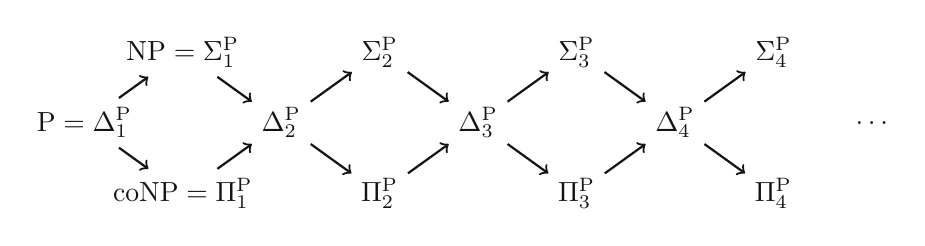
\begin{tikzpicture}[
    ph class/.style={
        font=\sffamily,
        text=black!92
    },
    ph inclusion/.style={
        ->,
        thick,
        draw=black!92
    }
]
    % Mittlere Ebene (Delta-Klassen)
    \node[ph class] (delta1) at (0,0)
        {$\mathrm{P} = \Delta_{1}^{\mathrm{P}}$};
    \node[ph class] (delta2) at (2.5,0)
        {$\Delta_{2}^{\mathrm{P}}$};
    \node[ph class] (delta3) at (5,0)
        {$\Delta_{3}^{\mathrm{P}}$};
    \node[ph class] (delta4) at (7.5,0)
        {$\Delta_{4}^{\mathrm{P}}$};
    \node[ph class] at (10,0) {$\ldots$};

    % Obere und untere Ebenen (Sigma- und Pi-Klassen)
    \node[ph class] (sigma1) at (1.25,0.9)
        {$\mathrm{NP} = \Sigma_{1}^{\mathrm{P}}$};
    \node[ph class] (pi1) at (1.25,-0.9)
        {$\mathrm{coNP} = \Pi_{1}^{\mathrm{P}}$};

    \foreach \level/\xpos in {2/3.75,3/6.25,4/8.75} {
        \node[ph class] (sigma\level) at (\xpos,0.9)
            {$\Sigma_{\level}^{\mathrm{P}}$};
        \node[ph class] (pi\level) at (\xpos,-0.9)
            {$\Pi_{\level}^{\mathrm{P}}$};
    }

    % Pfeile bezeichnen Mengeninklusionen; alle verlaufen von links nach rechts.
    \foreach \level in {1,...,4} {
        \draw[ph inclusion] (delta\level) -- (sigma\level);
        \draw[ph inclusion] (delta\level) -- (pi\level);
    }
    \foreach \level/\nextlevel in {1/2,2/3,3/4} {
        \draw[ph inclusion] (sigma\level) -- (delta\nextlevel);
        \draw[ph inclusion] (pi\level) -- (delta\nextlevel);
    }
\end{tikzpicture}

    \caption[Beziehungen zwischen Komplexit\"atsklassen]{Beziehungen zwischen
    Komplexit\"atsklassen; Pfeile bezeichnen
    Mengeninklusionen. Adaptiert nach
    \cite[Abb.~6.1]{rapberger:2023:unpacking-argument}.}
    \label{fig:polynomielle-hierarchie}
\end{figure}

Anschaulich spiegeln die Ebenen
\(\Sigma_k^{\mathrm{P}}\) und \(\Pi_k^{\mathrm{P}}\)
verschachtelte existenzielle und universelle Entscheidungen wider.
Um die Schwierigkeit von Problemen vergleichen und Härteergebnisse
übertragen zu können, verwenden wir polynomielle Reduktionen.
\begin{Definition}[Polynomielle Reduktion]
    \label{def:polynomial-reduction}
    Seien \(Q\subseteq D_Q\) und \(Q'\subseteq D_{Q'}\)
    Entscheidungsprobleme. Das Problem \(Q'\) ist
    \emph{polynomiell auf \(Q\) reduzierbar}, geschrieben
    \(Q'\leq_{\mathrm{P}}Q\), wenn eine in polynomieller Zeit
    berechenbare Funktion \(R\colon D_{Q'}\to D_Q\) existiert, sodass
    für jedes \(x\in D_{Q'}\) gilt:
    \(x\in Q'\) genau dann, wenn \(R(x)\in Q\) gilt. Die Funktion \(R\)
    heißt eine \emph{polynomielle Many-one-Reduktion} von \(Q'\) auf~\(Q\).
\end{Definition}
Kurz gesagt übersetzt \(R\) positive Instanzen von \(Q'\) in positive
Instanzen von \(Q\) und ebenso negative Instanzen in negative Instanzen.
Im Folgenden sprechen wir vereinfachend von polynomiellen Reduktionen,
welche die Grundlage der folgenden Härte- und Vollständigkeitsbegriffe bilden. 

\begin{Definition}[Härte und Vollständigkeit]
    \label{def:hardness-completeness}
    Sei \(\mathcal{C}\) eine Komplexitätsklasse. Ein
    Entscheidungsproblem \(Q\) heißt \emph{\(\mathcal{C}\)-hart}, wenn
    für jedes Problem \(Q'\in\mathcal{C}\) die Beziehung
    \(Q'\leq_{\mathrm{P}}Q\) gilt. Das Problem \(Q\) heißt
    \emph{\(\mathcal{C}\)-vollständig}, wenn \(Q\)
    \(\mathcal{C}\)-hart ist und zusätzlich \(Q\in\mathcal{C}\) gilt.
\end{Definition}
Für einen \(\mathcal{C}\)-Härtebeweis genügt es somit, ein bereits
\(\mathcal{C}\)-hartes Problem auf das untersuchte Problem zu reduzieren.
Als Ausgangsprobleme dienen in dieser Arbeit insbesondere die beschränkten
QBF-Wahrheitsprobleme. Ihre Komplexität wird
durch Anzahl und Reihenfolge der Quantorenblöcke bestimmt.
\begin{Definition}[Beschränkte QBF-Wahrheitsprobleme]
    \label{def:bounded-qbf-truth}
    Sei \(k\geq 1\), seien \(X_1,\dots,X_k\) paarweise disjunkte,
    nichtleere Mengen boolescher Variablen und seien
    \(Q_1,\dots,Q_k\in\{\exists,\forall\}\) Quantoren mit
    \(Q_i\neq Q_{i+1}\) für jedes \(1\leq i<k\). Eine geschlossene QBF
    der Form
    \(\Phi=Q_1X_1\cdots Q_kX_k\,\varphi\), wobei \(\varphi\) eine
    quantorenfreie propositionale Formel über
    \(X_1\cup\cdots\cup X_k\) ist, besitzt \(k\)
    \emph{alternierende Quantorenblöcke}.

    Das beschränkte QBF-Wahrheitsproblem
    \(\mathrm{QBF}^{\exists}_k\) enthält genau die wahren Formeln dieser
    Form mit \(Q_1=\exists\). Das beschränkte QBF-Wahrheitsproblem
    \(\mathrm{QBF}^{\forall}_k\) enthält genau die wahren Formeln dieser
    Form mit \(Q_1=\forall\).
\end{Definition}
Für eine Variablenmenge \(X_i\) steht \(Q_iX_i\) für einen Block, in dem
alle Variablen aus \(X_i\) mit \(Q_i\) quantifiziert werden.

Der Index \(k\) gibt somit die Anzahl der Quantorenblöcke an, während der
Hochindex den äußersten Quantor bezeichnet. Diese Problemfamilien
charakterisieren die Ebenen der polynomiellen Hierarchie.
\begin{Theorem}[QBF-Vollständigkeit \parencites{meyer:stockmeyer:1972:equivalence-regex}
    {stockmeyer:meyer:1973:word-problems}]
    \label{thm:qbf-ph-completeness}
    Für jedes \(k\geq 1\) ist
    \(\mathrm{QBF}^{\exists}_k\)
    \(\Sigma_k^{\mathrm{P}}\)-vollständig und
    \(\mathrm{QBF}^{\forall}_k\)
    \(\Pi_k^{\mathrm{P}}\)-vollständig bezüglich polynomieller
    Reduktionen.
\end{Theorem}
Das Theorem liefert damit kanonische Ausgangsprobleme für die späteren
Härtebeweise. Auf der Seite der Argumentationssysteme bilden Verifikation
sowie kredulöse und skeptische Akzeptanz die grundlegenden
Vergleichsprobleme.
\begin{Definition}[Entscheidungsprobleme für AFs]
    \label{def:standard-af-problems}
    Sei \(F=(A,R)\) ein AF und sei
    \(\sigma\in
    \{\mathsf{gr},\mathsf{co},\mathsf{st},\mathsf{pr}\}\).
    Das \emph{Verifikationsproblem}
    \(\mathrm{VER}_{\sigma}\) fragt für ein gegebenes Labelling
    \(\lambda\colon A\to\mathcal{L}\), ob
    \(\lambda\in\Lambda_{\sigma}(F)\) gilt.
    Das Problem der \emph{kredulösen Akzeptanz}
    \(\mathrm{CRED}_{\sigma}\) fragt für ein gegebenes Argument
    \(a\in A\), ob
    \(
        \exists\lambda\in\Lambda_{\sigma}(F)\colon
        \lambda(a)=\mathsf{in}
    \)
    gilt. 
    Das Problem der \emph{skeptischen Akzeptanz}
    \(\mathrm{SKEPT}_{\sigma}\) fragt entsprechend, ob
    \(
        \forall\lambda\in\Lambda_{\sigma}(F)\colon
        \lambda(a)=\mathsf{in}
    \)
    gilt.
\end{Definition}
Verifikation prüft somit ein konkret vorgegebenes Labelling, kredulöse
Akzeptanz quantifiziert existenziell und skeptische Akzeptanz universell
über die \(\sigma\)-Labellings. Die bekannten Komplexitätsergebnisse sind
in Tabelle~\ref{tab:complexity-af-semantics} zusammengefasst
\parencite[Tab.~3.3]{dvorak:2012:computational-aspects}.
\begin{table}[h]
    \centering
    \caption{Komplexität der Verifikation sowie der kredulösen und
    skeptischen Akzeptanz für die betrachteten AF-Semantiken.}
    \label{tab:complexity-af-semantics}
    \small
    \begin{tabular}{@{}lcccc@{}}
        \toprule
        & \(\mathsf{gr}\)
        & \(\mathsf{co}\)
        & \(\mathsf{st}\)
        & \(\mathsf{pr}\) \\
        \midrule
        \(\mathrm{VER}_{\sigma}\)
            & in \(\mathrm{P}\)
            & in \(\mathrm{P}\)
            & in \(\mathrm{P}\)
            & \(\mathrm{coNP}\)-vollständig \\
        \(\mathrm{CRED}_{\sigma}\)
            & in \(\mathrm{P}\)
            & \(\mathrm{NP}\)-vollständig
            & \(\mathrm{NP}\)-vollständig
            & \(\mathrm{NP}\)-vollständig \\
        \(\mathrm{SKEPT}_{\sigma}\)
            & in \(\mathrm{P}\)
            & in \(\mathrm{P}\)
            & \(\mathrm{coNP}\)-vollständig
            & \(\Pi_2^{\mathrm{P}}\)-vollständig \\
        \bottomrule
    \end{tabular}
\end{table}
